
\chapter{$L^P$ and Lipschitz Estimates}\label{chap5}%chap 5

OUR\pageoriginale AIM IN  this chapter is to study how to measure the smoothing
properties of pseudo differential operators of non positive order in
terms of various important function spaces. Most of the interesting
results are obtained by considering operators of order $ - \lambda $
with  $ 0 \leq \lambda \leq n$. Indeed, if $P \epsilon \Psi ^{-
  \lambda} $ with $ \lambda > n $ and $ K (x,y)$ is the  distribution
kernel of $P$ then, by  Theorem \ref{chap4:sec2:thm4.10} we know that
$ K \epsilon 
C^j \Omega \times \Omega )$ when $j < \lambda -n$. So these operators
can be studied by elementary methods. What is more, when  $P
\epsilon  \Psi ^{-\lambda}, D ^ {\alpha} P \epsilon \Psi ^{-
  \lambda + | \alpha |}$.  So, by a proper choice of $\alpha$,  we can
make $0 \leq \lambda - | \alpha | \leq n $ and then study $ D^ \alpha
P $ rather than $P$ itself.  Actually, we shall restrict attention to
operators of order $- \lambda $ where $ 0 \leq \lambda < n $. The
transitional case $\lambda = n$ requires a separate treatment to
obtain sharp  results; however,  for many purpose, it suffices  to
make the trite observation  that an operator of order $-n$ can be
regarded as an operator of order $-n + \epsilon $. Further, we
restrict our attention to  $\Psi DO's$ whose symbols have asymptotic
expansions  
$$
p (x, \xi ) \sim \sum_{j=0}^{\infty} p_j (x,\xi )
$$
where  $P_j$ is homogeneous of degree $- \lambda - j $. (These $p_j '
s$ no  longer belong to our symbol classes, being   singular at $\xi
=0$,  but we can  still consider the operators $p_j (x,D)$.) By the
preceding remarks, it will  suffice to consider the operators
corresponding to the individual terms\pageoriginale in the series $ \sum p
_j$ whose degrees of homogeneity are  between $0$ and $- n$. Thus we
are looking at $p(x, D)$ where $p(x, \xi)$ is $C^{\infty}$ on $
\mathbb{R}^n \times 
\mathbb{R}^n \backslash\{0\}$ and homogeneous of degree $-\lambda $ in
$\xi $ where $ 0\leq \lambda < n$. 

Since $\lambda < n$, for each $x, p(x,.) $ is locally integrable at
the origin and hence defines a tempered distribution. Denoting the
inverse Fourier transform of this distribution  $p_2^\vee (x,.)$ we
then have 	 
\begin{align*}
  p(x,D)  u  (x) &= \int e^{2 \pi i x. \xi } p(x, \xi ) \hat{u}(\xi) d \xi\\
  &= (p_2^{ \vee }(x,.) * u) (x)\\
  &= \int p_2^{\vee} (x, x-y) u (y) dy.
\end{align*}

Thus  we see that the distribution kernel of $p(x,D)$ is given by $K
(x, y)\break = p^v_{2} (x, x-y)$. 

Let us digress a little to make some remarks  on homogeneous distributions.

\begin{defi}%def 5.1
  A distribution  $f \epsilon S'$ is said to be {\em homogeneous of
  degree} $ \mu,  if < f,  \phi _r > = r^ \mu < f, \phi > $  for all
$\phi \epsilon S$ where $\phi _r$   is the function defined by
$\phi _r (x) = r^{-n}   \phi (x/r)$. 
\end{defi}

\noindent \textbf{Exercise.}
  \begin{enumerate}
  \item Show that the above definition agrees with the usual definition
    of homogeneity  when $f$ is a locally integrable function. 
  \item Show that if $f \epsilon S'$  is homogeneous of degree $\mu
    $, then $D^\alpha f$ is homogeneous of degree $\mu - | \alpha|$. 
  \item Show\pageoriginale that $D^\alpha \delta $ is homogeneous of degree $-n- |
    \alpha |$  (where $\delta$ is the Dirac measure at 0). 
  \end{enumerate}

Let us now prove a proposition concerning the Fourier transform of
homogeneous distributions. It turns out that the Fourier transform of
such a distribution is also  a homogeneous one. Precisely, we have the
following 

\setcounter{prop}{1}
\begin{prop}\label{chap5:prop5.2}%pro 5.2
  If $f$ is a tempered distribution, homogeneous of degree $\mu$,
  then $\hat{f}$  is homogeneous of degree $-\mu -n$. If $f$ is also
  $C^ \infty$ away from the origin,  then the same is true  of
  $\hat{f}$. 
\end{prop}

\noindent \textit{Proof}
  If $f$ is homogeneous of degree $\mu$, then for $\phi \epsilon S$ 	
  \begin{align*}
    < \hat{f}, \phi_r > &= <f, ( \phi _r ) \hat { } > = < f, r ^{-n}
    \hat{\phi}_{1/r}> = r^{-n- \mu }  <  f, \hat{\phi}>\\ 
    & = r^{- \mu -n }< \hat{f},  \phi >.\tag*{$\Box$}
  \end{align*}

 This proves the first assertion. To prove the second assertion,
 choose $\phi \epsilon C^\infty_0 $ with $\phi = 1$ in a
 neighbourhood of the origin and write $ f= \phi f + (1- \phi )f$.
 Since $ \phi f \epsilon E ', ( \phi f) \hat { } $ is $ C^\infty $
 everywhere. On the other  hand,  $(1 - \phi )f$ is $C^\infty$ and
 homogeneous of degree $\mu$ for large  $\xi$,  and hence lies in $S^
 \mu ( \mathbb{R}^n)$. Let $p(x, \xi ) = (1 - \phi ) ( \xi ) f ( \xi
 )$. The distribution kernel of $p(x,D)$ is given by  
 \begin{align*}
   K(x,y) &= \int e^{-2 \pi i (y-x),\xi} (1 - \phi ) ( \xi ) f  ( \xi) d\xi\\
   &= ((1 - \phi ) f)\hat { } (y-x).
 \end{align*} 
 
 
 Since $K$ is $C^{\infty}$ away from the diagonal, we see that $((1-
 \phi ) f) \hat { } $ is $C^{\infty}$ away from the origin. Hence
 $\hat{f} $ is $C^\infty $ on $\mathbb{R}^n \backslash \{0\}$. 
 
 Returning\pageoriginale to our operators $p(x, D) $ with $p( x,\xi )$ homogeneous
 of degree $- \lambda $ in $ \xi,  0 \leq \lambda < n$, by the
 proposition above, we have 
 $$
 p(x,D)u= \int K (x, x-y) u (y) dy 
 $$
  where $K= P _2^\vee$ is $C^ \infty $ on $ \mathbb{R}^n \times
  \mathbb{R}^n \backslash \{0\}$ and homogeneous of degree $\lambda-n
  $ in the second variable. 
 
 Finally, we restrict attention to constant coefficient case, i.e.,
 $K(x, x-y) = K (x-y)$. The essential  ideas are already present in
 this case and the results we shall obtain can be generalised to the
 variable coefficient case in a rather routine fashion. Let us give  a
 name  to the objects we are finally going to study.  
 
\setcounter{defi}{2}
\begin{defi}\label{chap5:def5.3}%def 5.3
  A tempered distribution $K$ which is homogeneous of 	  degree
  $\lambda -n $ and $C^\infty$ away from the origin is called 
    a kernel of type $\lambda$. If $K$ is a kernel of type $\lambda$,
  the operator $Tf= K * f $ is called an operator of type
  $\lambda$.   
\end{defi} 
 
 We now classify the kernels of type $\lambda \ge 0$.
\setcounter{prop}{3}
 \begin{prop}\label{chap5:prop5.4}%pro 5.4
   Suppose $\lambda > 0$ and $f \epsilon C ^\infty (
  \mathbb{R}^n \backslash \{0\})$ is homogeneous of degree $\lambda -n
  $ in the sense of functions. Then $f$ is locally integrable and
  defines a distribution $F$  which is a kernel of type $\lambda$. 
 \end{prop} 
 
 \textit{Conversely, if $F$ is a kernel of type $\lambda$ and  $f$ is
   the function with which $F$ agrees on $\mathbb{R}^ n \backslash
   \{0\}$,then $< F,  \phi > = \int f \phi $ for every $\phi $ in
   $S$.} 
 
 \begin{proof}
   Since $\lambda > 0 $, $f$ is locally integrable and of (at most )
   polynomial growth at $\infty$, so $f$ defines an $F$ in $S'$. It is
   easy to check that $F$ is homogeneous in the sense defined above, 
   i.e.$ < F, \phi _r > = r^{\lambda-n}<F, \phi >$,\pageoriginale and so $F$ is a
   kernel of type $\lambda$. 
 \end{proof}
 
For the converse, define $G$ by $< G, \phi > = <  F, \phi > - \int f
\phi, \phi \in S$.  
Then $G$ is a distribution supported at $0$ and hence we have $G =
\sum c_ \alpha  D^\alpha  \delta$. Therefore, 
$$
< G, \phi _r > = \sum c_ \alpha r^{-n- | \alpha|} (D^\alpha \phi)
(0) = O (r^{-n}), ~\text{as}~ r \to \infty.
$$
 
On the other hand, 
  $$
 < G, \phi_r > = r ^{-n-\lambda}<G, \phi>
 $$
 and this is not $O(r^{-n})$ as $r$ tends to $\infty$ unless $< G,
 \phi > = 0$. Hence $G= 0$ and this completes the proof. 
 
 Suppose that $f \epsilon C^ \infty ( \mathbb{R}^n \backslash
 \{0\})$ is homogeneous of degree $-n$. Then $f$ is not locally
 integrable near $0$ and so does not define a distribution in a
 trivial way. However,  let us define  
 $$
 \mu _f = \int\limits_{| x| =1} f(x) d \sigma (x).		
 $$

  If $\mu _f = 0$ there is a canonical distribution associated with
  $f$ which is called \textit{principal value } of $f, PV(f)$, defined
  by  
  $$
  < PV (f), \phi > = \lim_{ \epsilon \to 0  } \int\limits_{| x| >
    \epsilon} f(X) dx. 
  $$
  
  To see that this limit exists, we observe that 
  $$
  \int\limits_{\epsilon < | x| < 1} f(x) dx = \mu _f
  \int\limits_{\epsilon}^{1} r^{-1} dr = 0. 
  $$
  
  Hence
  $$
  < PV (f), \phi > = \lim_{\epsilon \rightarrow 0}
  \int\limits_{\epsilon < | x | < 1} f(x) (\phi (x) - \phi (0)) dx
  + \int\limits_{| x| \ge 1} f(x) \phi (x) dx, 
  $$
 where\pageoriginale the last integrals are absolutely convergent, since
\begin{gather*}
  | \phi (x) - \phi (0) | \le c |x|, \qquad \text{so that}\\
  \int\limits_{|x| < 1} | f ( x) || \phi (x) - \phi (0)| dx \le c
  \int\limits_{|x| < 1} | x |^{-n+1} dx < \infty. 
\end{gather*}

Further, the estimate on $\phi (x) - \phi (0)$ depends only on the
first derivatives of $\phi$ via the mean value theorem, so it is
easily verified that the functional $PV(f)$ is continuous on
$S$. Finally, we observe that  
\begin{align*}
  < PV (f), \phi_r > &= ~ \lim_{\epsilon \to 0} \int\limits_{|x| >
    \epsilon} f(x) r^{-n} \phi (x/r) dx\\ 
  & = ~ \lim_{\epsilon \to 0} \int\limits_{|y| > (\epsilon/r)}
  f(y) r^{-n} \phi (y) dy\\ 
  & = ~ r^{-n} < PV (f), \phi >.
\end{align*}

Thus $PV (f)$ is homogeneous of degree -$n$ and so is a kernel of type 0.

The following theorem gives a sort of converse to the above results.

\setcounter{thm}{4}
\begin{thm}\label{chap5:thm5.5}%the 5.5
  Suppose $F$ is a kernel of type $0$ and $f$ is
    the function with which $F$ agrees on $\mathbb{R}^n \backslash  \{
  0\}$. Then $\mu_f = 0$ and  $F = PV(f) + c \delta$, 
    for some constant $c$. 
\end{thm}

\noindent\textit{Proof.}
Define the functional $G$ on $S$ by
\begin{equation*}
  < G, \phi > = \int\limits_{|x| \le 1} f(x) (\phi (x)-(\phi (0)) dx +
  \int\limits_{|x| > 1} f(x) \phi (x) dx. \tag*{$\Box$}
\end{equation*}

By the same argument as above, $G$ is a tempered distribution and $G =
F$ on $\mathbb{R}^n / \{ 0\}$. Therefore, $G -  F = \sum c_{\alpha}
D^{\alpha} \delta$. Now, $< F, \phi_r > = r^{-n} < P, \phi >$ so that  
$$
< G, \phi_r > - r^{-n} <G, \phi > = < G-F \phi_r > - r^{-n} < G - F,
\phi > = 0 (r^{-n}) 
$$
as\pageoriginale $r$ tends to $\infty$. On the other hand, for $r > 1$,
\begin{align*}
  < G, \phi_r > &- r^{-n} < G, \phi > = \int\limits_{|x| \le 1/r} r^{-n}
  f(x) (\phi (x) - \phi (0)) dx \\
  & + \int\limits_{|x| > 1/r} r^{-n} f(x)
  \phi (x) dx - r^{-n} \int\limits_{|x| \le 1} f(x) (\phi (x) - \phi
  (0)) dx-r^{-n} \\
  & \hspace{5cm}\int\limits_{|x| > 1} f(x) \phi (x) dx\\ 
  & = r^{-n} \phi (0) \int\limits_{1r \le |x| \le 1} f(x) dx = r^{-n}\phi
  (0) \log r \mu_{f'} ~\text { for every }~ \phi. 
\end{align*}


This is not $0 (r^{-n})$ as $r$ tends to $\infty$ unless $\mu_f =
0$. Finally, $F- PV (f)$ is a kernel of type $0$ which is supported at
the origin and hence is a multiple of $\delta$. 

To study the boundedness of operators of type $\lambda$ on $L^p$
spaces, we need some concepts from measure theory. 

\setcounter{defi}{5}
\begin{defi}\label{chap5:def5.6}%def 5.6
  Let $F$ be a measurable function defined on
  $\mathbb{R}^n$. Then the distribution function of $f$ is
  the function  $\delta_f : (0, \infty) \to [0, \infty]$ given
  by $\delta_f(t) = |E_t|$, where  $E_t = \{ x: |f (x) | >
  t\}$. 
\end{defi}

From the distribution function of $f$, we can get a large amount of
information regarding $f$. For example, we have  
$$
\int |f(x) |^p dx = - \int\limits_{0}^{\infty} t^p d \delta_f (t)
$$
(To see this, observe that the Riemann sums for the Stieltjes integral
on the right are approximating sums for the Lebesque integral on the
left). 

If $t^p \delta_f (t)$ converges to $0$ as $t$ tends to 0 and $t$
tends to $\infty$, we can integrate by parts to obtain $\int | f (x)
|^p dx = p \int\limits_{0}^{\infty} t^{p-1} \delta_f (t) dt$. 

Using\pageoriginale the concept of distribution functions, we will now
define weak $L^p$ spaces. 

\begin{defi}\label{chap5:def5.7}%def 5.7
  For $1 \le p < \infty$ we define weak  $L^p$ as $\{ f: \delta_f
  (t) \le (c/t)^p$ for some constant $c \}$. For $f \epsilon$ weak
  $L^p$, the smallest such constant $c$ will be denoted by
  $[f]_p$. Thus, if $f \epsilon $weak $L^p$, we have   
  $$
  \delta_f(t) \le ( [f]_p/t)^p.
  $$
\end{defi}

For $p = \infty$, we set weak $L^{\infty} =  L^{\infty}$.

\setcounter{prop}{7}
\begin{prop} \label{chap5:prop5.8}% pro 5.8
CHEBYSHEV 'S INEQUALITY) $L^p \subset$ weak $L^p$ and $[f]_p \le
  || f ||_p$. 
\end{prop}

\begin{proof}
  For $f \epsilon L^p $, if $E_t = \{ x: |f (x) | > t \}$,
  $$
  || f ||^p_p = \int\limits_{\mathbb{R}^n} | f(x) |^p dx \ge
  \int\limits_{E_t} |f (x) |^p dx \ge t^p |E_t| 
  $$
  i.e., \quad $| E_t | \le (|| f ||^{p}/t) p$.
  
  From this, it follows that $f \epsilon$ weak $L^p$ and $[f]_p \le
  || f ||_p$. 
\end{proof}

\setcounter{rem}{8}
\begin{rem} \label{chap5:rem5.9}%rem 5.9
  It is not true that $L^p =$ weak $L^p$ for $1 \le p < \infty$. For
  example, $f(x) = |x|^{-n/p}$ belongs to weak $L^p$ but not $L^p$. 
\end{rem}

\begin{rem}\label{chap5:rem5.10} %rem 5.10
The function $f \to [f]_p$ satisfies $[cf]_p = |c| [f]_p$. 
\end{rem}

But it fails to satisfy triangle inequality and hence is not a
norm. However, since 
$$
\{ |f +g | > t \} \subset \{|f| t/2 \} \cup \{|g | > t/2 \},
$$
we have
$$
\delta_{f+g} (t) \le \delta_f (t/2) + \delta_g (t/2)
$$
which\pageoriginale gives, when $f$ and $g$ are in weak $L^p$,
\begin{gather*}
  \delta_{f+g} (t) \le (2^p [f]^p_p + 2^p [g]^p_p)/t^p  ~ \text {so that}\\
        [f + g]_p \le 2([f]^p_p + [g]^p_p)^{1/p} \le 2([f]^p + [g]_p).
\end{gather*}

The functional $[.]_p$ thus defines a topology on weak $L^p$ which
will turn it into a (non-locally convex) topological vector space.  

\setcounter{defi}{10}
\begin{defi} \label{chap5:def5.11}%def 5.11
  A linear operator $T$ defined on a space of functions is said to be of
  {\em weak type} $(p, q), 1\le  p, q \le \infty$, if $T$ is a bounded linear
  operator from $L^p$ into weak $L^q$, i.e. for every $f \epsilon
  L^p, [Tf]_q \le c || f ||_p$ for some constant $c$ independent of
  $f$. 
\end{defi}

\textit { We will now state the Marcinkiewicz interpolation theorem
  and use it to prove generalisations of Young's inequality (Theorem
  \ref{chap1:sec1:thm1.3}). } 

\setcounter{thm}{11}
\begin{thm}[J. Marcinkiewicz]\label{chap5:thm5.12} % the 5.12
  Suppose  $T$ is of weak types  $
  (p_o, q_o) $ and $(p_1, q_1)$ with $1 \le p_i \le q_i
  \le \infty$, $p_0 < p_1, q_0 \neq q_1$, i.e., $['\Gamma f]^{q_i} \le
  c_i || f ||_{p_i}$ for  $i = 0, 1$. Then,  if  
$$
1/p_{\theta} = (1-\theta)/p_0 + (\theta/p_1), 1/q_{\theta} =
(1-\theta)/q_0 + (\theta/q_1), 0 < \theta < 1, 
$$
$T$ is bounded from $L^{p_{\theta}}$ to $L^{q_{\theta}}$ i.e., $|| Tf
||_{q_{\theta}} \le c_{\theta} || f ||_{p_{\theta}}$ where {\em the
  constant } $c_{\theta}$ {\em depends only on} $p_0, q_0, p_1, q_1,
c_0, c_1$ and $\theta$. 
\end{thm}

\textit {For the proof of this theorem}, see $A$. Zygmund \cite{5} or
E.M.Stein \cite{2}.
 
\setcounter{thm}{12}
\begin{thm}[GENERAL FROM OF YOUNG'S
    INEQUALITY]\label{chap5:thm5.13}  
  If $(1/p) + (1/q) - 1 =
  1/r, 1 \le p, q, r< \infty$, Then, for $f \epsilon L^p, g
  \epsilon L^q f * g \epsilon L^r$ and we have $|| f * g
  ||_r \le c_{pq} || f ||_p || g||_q$.  
\end{thm}

(In\pageoriginale fact, $c_{pq} \le 1$ for all $p, q$, although our
proof does not yield this estimate).
 
\begin{proof}%pro
  Fixing $f \epsilon L^p$, consider the convolution operator $g \to
  T_q = f * g$. We know that for $g \epsilon L^1, Tg \epsilon L^p$
  and $|| Tg ||_p \le || f ||_p || g ||_1$. Further if $p'$ is the
  conjugate of $p$, then, by H\"{o}lder's inequality $|| Tg ||_{\infty}
  \le || g ||_p, || f ||_p$ for $g \epsilon L^{p'}$. Thus we see that
  the operator $T $ is of weak types $(1, p)$ and $(p',
  \infty)$. Therefore, by the Marcinkiewicz interpolation theorem, $T$
  maps $L^{p_{\theta}}$ boundedly into $L^{q_{\theta}}$ for every $0 <
  \theta < 1$ with 
  $$
  (1/p_{\theta}) = 1 - \theta + (\theta/p') = 1 -  (\theta/p) \text{
    and } 1/q_{\theta} = (1/p) - \theta/p. 
  $$ 
\end{proof}

Given $r$ with $(1/p) + (1/q) - 1 =  (1/r)$, set $q_{\theta =
  r}$. Then $(1/p_{\theta})  = 1 +  (1/r) - (1/p) = (1/q)$. Hence we
get the required result. 

\setcounter{thm}{13}
\begin{thm}[WEAK TYPE YOUNG'S INEQUALITY]\label{chap5:thm5.14} 
  Let $1 \le p < q < \infty$,
  $(1/p) + (1/q) > 1$ and  $(1/p) + (1/q) - 1 = (1/r)$. 
  Suppose $f \epsilon L^p$ and $g \epsilon $ weak
  $L^q$. Then, we have 
  \begin{enumerate}[a)]
  \item $f * g$ exists a.e. and is in weak $L^r$, and
    $$
    [f * g ]_r \le c_{pq} || f ||_p [g]_q
    $$
  \item If $p > 1$, then $f * g \epsilon L^r$ and $||f * g ||_r \le
    c'_{pq} || f ||_p [g]_q$. 
  \end{enumerate}
\end{thm}

\begin{proof}%pro
  \begin{enumerate}[a)]
  \item It suffices to assume that $|| f ||_p = [g]_p = 1$ and to show
    that $[f * g]_r \le c_{pq}$. Given $\alpha > 0$, let 
    $$
    M = (\alpha/2)^{p'/(p'-q)} (p'/(p'-q)^{-1/(p'-q)}
    $$
    where $p'$ is as usual the conjugate of $p$. Define
    \begin{align*}
      g_1 (x) & = ~ g(x), \text { if } | g (x) | > M\\
      & = ~ 0 \text { otherwise}\\
      and \qquad g_2(x) & = ~ g(x) - g_1 (x). \qquad \text { Then }
    \end{align*}\pageoriginale
    $$
    \delta_{f * g} (\alpha) \le \delta_{f * g_1} (\alpha/2) + \delta_{f *
      g_2} (\alpha/2) 
    $$
    and we shall estimate the quantities on the right separately. By
    Holder's inequality, 
    $$
    || f * g_2 ||_{\infty} \le || f ||_p || g_2 ||_{p'} = || g_2 ||_{p'}.
    $$
        
    Since $(1/q) - (1/p') = 1/r > 0$, we see that $p' -  q > 0$, and hence 
    \begin{align*}
      || g_2 ||^{p'}_{p'} & = ~ p' \int\limits_{0}^{\infty} t^{p' - 1}
      \delta_{g_2} (t) dt\\ 
      & = ~ p' \int\limits_{0}^{M} t^{p' - 1} (\delta_g (t) - \delta_g (M)) dt\\
      & \le ~ p' \int\limits_{0}^{M} t^{p' - 1} t^{-q_{dt}} = (p'/(p'-q))
      M^{p' - q} = (\alpha/2)^{p'}. 
    \end{align*}
    
    Thus $(f * g_2) (x)$ exists at all points and $|| f * g_2 ||_{\infty}
    \le \alpha/2$. 
    
    Consequently $\delta_{f * g_2} (\alpha/2) = 0$. Next consider
    \begin{align*}
      || g_1 ||_1 & = ~ \int\limits_{0}^{\infty} \delta_{g_1} (t) dt =
      \int\limits_{0}^{M} \delta_g (M) dt + \int\limits_{M}^{\infty}
      \delta_g (t) dt \\ 
      & \le ~ \int\limits_{0}^{M} M^{-q} dt + \int\limits_{M}^{\infty}
      t^{-q} dt. 
    \end{align*}
    
    The integral $\int\limits_{M}^{\infty} t^{-q} dt$ converges since $q >
    1$, and we obtain  
    $$
    || g_1 ||_1 \le M^{1-q}+M^{1-q}/(q-1) = (q/(q-1)) M^{1-q}.
    $$
    
    Also, by Chebyshev inequality,
    \begin{align*}
    \delta_{f * g_1} \left(\frac{\alpha}{1}\right) & \le \left(\frac{|| f *
      g_1 ||}{\alpha/2} p\right) p \\
      & \le  (2^p/\alpha^ p) (q/(q-1))^p (\alpha/2)^{\frac{p'}{p'-q} p(1-q)}
      (p'/(p'-q))^{-\frac{p(1-q)}{p'-q}}\\ 
      & = c_{pq} \alpha^{-r}
    \end{align*}\pageoriginale
  
    Hence $(a)$ is proved.
  \item The operator $f \to f * g$ is of weak type $(1, q)$ by
    $(a)$. Also, if we choose $\bar{p} > p$ with $(1/\bar{p})+ (1/q) >
    1$ and put $(1\bar{r}) =  (1/\bar{p}) + (1/q) - 1$ then by $(a)$, $f
    \to f * g$ is of weak type $(\bar{p}, \bar{r})$. Therefore, by
    Marcinkiewicz, $f \to f * g$ is bounded from $L^p$ into
    $L^{q_{\theta}}$ with 
    $$
    1/p_{\theta} = 1 -  \theta + (\theta/\bar{p}), ~ (1/q_{\theta}) =
    ((1-\theta)/q) + ~ (\theta/\bar{r}). 
    $$
  \end{enumerate}
    Putting $q_{\theta} = r $ we get  $p_{\theta} = p$. Hence $T$ maps
    $L^p$ continuously to $L^r $ and $|| f * g ||_r \le c'_{pq} || f ||_p
    [g]_q$. 
\end{proof}

\setcounter{coro}{14}
\begin{coro}\label{chap5:coro5.15}%coro 5.15
  If  $T$ is an operator of type  $\lambda, 0 < \lambda <
  n$, then  $T$ is bounded from  $L^p$ into  $L^q$,
  whenever $1 < p < q < \infty$ and  $1/q = 1/p -
  \lambda/n$. Also, $T$ is of weak type $(1,
  n/(n-\lambda))$. 
\end{coro}

\begin{proof}
  If $K$ is a kernel of type $\lambda$, we have
  $$
  | K (x) | = |x|^{\lambda-n} K(x/|x| ) | \le c|x|^{\lambda-n},
  $$
  which implies that $K \epsilon $ weak $L^{n/
    (n-\lambda)}$. Therefore, by Theorem \ref{chap5:thm5.14}(b),
  if $f \epsilon 
  L^p$ and $Tf = K * f$ then $Tf \epsilon L^q$ where 
{\fontsize{10pt}{12pt}\selectfont
  $$
  (1/q) = (1/p) + ((n-\lambda(/n)-1 = (1/p)-(\lambda/n) \text { and } ||
  Tf ||_q \le c [f]_p \le c || f ||_p. 
  $$}\relax
\end{proof}

Also we see that $T$ is of weak type $(1, n/(n-\lambda))$ by Theorem
\ref{chap5:thm5.14} (a).  

The\pageoriginale limiting case of this result with $\lambda = 0$ is also true, but
this is a much deeper theorem: 

\setcounter{thm}{15}
\begin{thm}\label{chap5:thm5.16} % the 5.16
  (Calderon - Zygmund) Operators of type 0 are
    bounded on $L^p, 1 < p < \infty$. 
\end{thm}

\begin{proof} %pro
  Let $T$ be an operator of type 0 with kernel $K$ i.e., $Tf = K *
  f$. To begin with, we can regard $T$ as a map from $c^{\infty}_o$ to
  $c^{\infty}$ and we shall show that $|| Tf ||_p \le c_p || f||_p$ for
  $f \epsilon c^{\infty}_o$, $1 < p < \infty$, so that $T$ extends
  uniquely to a bounded operator on $L^p$.  
\end{proof}

We have $K = PV(k) + c \delta$ so that $Tf = PV (k) * f + cf$. Since
the identity operator is continuous, we shall assume that $c = 0$ and
also we shall identify $K$ with $k$. The proof now proceed in several
steps. 

\begin{step} \label{chap5:step1}% ste 1
  $T$ is bounded on $L^2$. Indeed, we have $(Tf) \hat{} t = \hat{k}
  \hat{f}. \hat{k}$ is smooth away from $0$ and homogeneous of degree
  $0$, hence is bounded on $\mathbb{R}^n$ Therefore, 
  $$
  || Tf ||_2 = || (Tf) \hat{~} ||_2 \le || \hat{k} ||_{\infty} || \hat{f}
  ||_2 = || \hat{k} ||_{\infty} || f ||_2. 
  $$
\end{step}

\begin{step} \label{chap5:step2}%ste 2
  Fix a radial function $\phi \epsilon c^{\infty}_o$ with $\phi (x) =
  1$ for $|x| \le \dfrac{1}{2}$ and $\phi (x) = 0$ for $|x| \ge 1$. For
  $\epsilon > 0$, we define $k_{\epsilon} (x) = k(x) (1-\phi
  (x/\epsilon))$ and $T_{\epsilon} f = k_{\epsilon} * f$. Then
  we claim that $T_{\epsilon}$ is bounded on $L^2$ uniformly in
  $\epsilon$. To see this, we observe that 
  \begin{align*}
    (T_{\epsilon} f)\hat{} & = \hat{f} \hat{k}_{\epsilon} =
    \hat{f}(k - k \phi (x/\epsilon))\hat{}\\ 
    & = \hat{f} \hat{k} - \hat{f} (\hat{k } * (\phi
    (x/\epsilon))\hat{}) 
  \end{align*}
  which gives
  \begin{align*}
    || T_{\epsilon} f ||_2 & = || (T_{\epsilon} f)\hat{} ||_2 \le ||
    \hat{f} ||_2 || \hat{k} ||_{\infty} \{ 1 +  \epsilon^n \int |
    \hat{\phi} (\epsilon \xi) | d \xi  \}\\ 
    & = || f ||_2 || \hat{k} ||_{\infty} \{ 1+ || \hat{\phi} ||_1  \}
  \end{align*}
\end{step}

\begin{step}\label{chap5:step3} %ste 3
  $T_{\epsilon}$\pageoriginale is of weak type (1,1) uniformly in $\epsilon$.
  The proof of this is more involved and will be given later. 
\end{step}

\begin{step}\label{chap5:step4}% ste 4
  By steps \ref{chap5:step2} and \ref{chap5:step3}, using
  Marcinkiewicz, we get that $T_{\epsilon}$ 
  is bounded on $L^p$ for $1 < p < 2$ uniformly in $\epsilon$. 
\end{step}

\begin{step}\label{chap5:step5} % ste 5
  $T_{\epsilon}$ is bounded on $L^p$, for $2 < p < \infty$, uniformly
  in $\epsilon$. Indeed, for $f, g \epsilon C^{\infty}_o$, 
  $$
  \int (T_{\epsilon } f) ~ (x) ~ g(x) ~ dx = \int ~ f(x) ~
  (\tilde{T}_{\epsilon}g) ~ (x) ~ dx 
  $$
  with $\tilde{T}_{\epsilon} g ~ = ~ \tilde{k}_{\epsilon} * g$,
  $\tilde{k}_{\epsilon} = k_{\epsilon}(-x) = k (-x) (1- \phi
  (x/\epsilon))$. Since $\tilde{k}_{\epsilon}$ satisfies the same
  conditions as $k_{\epsilon}$, we see that $\tilde{T}_{\epsilon}$
  is bounded on $L^q$ for $1 < q < 2$ uniformly in $\epsilon$. So if
  $(1/p) +  (1/q) = 1$, $1 < q < 2$, 
  $$
  || T_{\epsilon} f||_p ~ = ~ \sup_{g ~ \epsilon ~ C^{\infty}_o}
  \frac{| \int (T_{\epsilon} f) g |}{|| g ||_q} ~ \le ~ \sup_{g
    \epsilon C^\infty_o} \frac{||
    \tilde{T}_{\epsilon} g ||_q}{|| g ||_q} ~ || f ||_p ~ = c || f
  ||_p. 
  $$
\end{step}

\begin{step}\label{chap5:step6}%step 6
  If $f \epsilon C^{\infty}_o$,  $T_{\epsilon} f$ converges to
  $Tf$ in the $L^p$ norm, $1 \le p \le \infty$ as $\epsilon$ tends to
  $0$. Since $\phi$ is radial and $\mu_k = 0$, 
  $$
  \int\limits_{| x | = r} \phi (x/\epsilon) k (x) d \sigma (x) = c
  \int\limits_{| x | = r} k (x) d \sigma (x) = 0; 
  $$
  so, for $\epsilon \le 1$, we have
  $$
  \displaylines{\hfill
  (T_{\epsilon}f) (x) ~ = ~\int\limits_{| y | \le 1} (f (x-y)-f(x)) ~
  k(y) (1-\phi (y/\epsilon)) dy + \int\limits_{|y | > 1} f(x-y) ~
  k(y) dy \hfill \cr
  \text{and hence} \hfill
  (T_{\epsilon} f) (x) - (Tf) (x) ~ = ~ \int\limits_{|y | \le
    \epsilon} f(x-y)-f(x) k(y) \phi (y/\epsilon) dy. \hfill }
  $$\pageoriginale
\end{step}

Now $\supp (T_{\epsilon} f - Tf) \subset \{ x: d(x, \supp f) \le
\epsilon \} \subset A$, a fixed compact set. Since, on compact
sets, the uniform norm dominates all $L^p$ norms, it suffices to show
that $(T_{\epsilon} f - Tf)$ converges to $0$ uniformly on $A$. But  
\begin{multline*}
  || T_{\epsilon} f - f ||_{\infty} \le || \grad f ||_{\infty}  ~
  \int\limits_{| y | \le \epsilon} c| y | |y |^{-n} dy \le c' ||
  \grad f ||_{\infty}\\ 
  \int\limits_{0}^{\epsilon} r^{1-n} r^{n-1} dr =
  c'' \epsilon \to 0, \text { as } \epsilon \to 0. 
\end{multline*}

\begin{step} \label{chap5:step7}% ste 7
  If $f \epsilon L^p$ and $\eta > 0$, choose $g \epsilon
  C^{\infty}_{o}$ with $|| g - f ||_p < \eta$. 
\end{step}


Then $|| T_{\epsilon} f - T_{\delta} f ||_p \le || T_{\epsilon}
(f-g)||_p + || T_{\epsilon} g - T_\delta g ||_p + ||T_\delta (g-f)
||_p \le 2c \eta + || T_{\epsilon}g - T_\delta g ||_p$. 


Since $\eta$ is arbitrary and $|| T_{\epsilon} g - T_\delta g ||_p$
converges to $0$ as $\epsilon$, $\delta$ tend to $0$ by
step \ref{chap5:step6},
we see that $(T_{\epsilon} f)$ is Cauchy in the $L^p$ norm. Setting 
$$
Tf = \lim_{\epsilon \to 0} T_{\epsilon} f, || Tf ||_p \le c || f ||_p.
$$

Thus the theorem is proved modulo Step \ref{chap5:step3}.

Let us now proceed to the proof of Step
\ref{chap5:step3}. First, we need a lemma which will be used in
the proof.  

\setcounter{lem}{16}
\begin{lem} \label{chap5:lem5.17}% lem 5.17
  Suppose  $F \epsilon L^1, F \ge 0$ and $\alpha >
  0$. Then there exists a sequence  $(Q_k)$ of closed cubes
  with sides parallel to the coordinate axes\pageoriginale and disjoint interiors
  such that 
  \begin{enumerate}[a)]
  \item $\alpha < \dfrac{1}{| Q_k |} \int\limits_{Q_k} F \le 2^n \alpha$
    for all  $k$, 
  \item If $\Omega = \bigcup\limits_{1}^{\infty} Q_k$, then $| \Omega |
    \le (1/\alpha) || F ||_1$, 
  \item $F(x) \le \alpha$ for a.e. $x \notin \Omega$. 
  \end{enumerate}
\end{lem}

\begin{proof} %pro
  Let $r = ( || F ||_1 / \alpha)^{1/n}$ and for $j = 1, 2, \ldots$ let
  $\mathscr{Q}_j$ be the collection of closed cubes of side length
  $r/2^j$ and vertices in $(r/2^j) \mathbb{Z}^n$. Our sequence will be
  constructed in the following way. Put those cubes $Q \epsilon
  \mathscr{Q}_1$ in the sequence which satisfy $\alpha < \dfrac{1}{| Q
    |} \int\limits_{Q} F$. Then 
  $$
  \frac{1}{|Q|} \int\limits_{Q} F \le \frac{1}{| Q |} || F ||_1 = (2^n
  \alpha/ || F ||_1) || F ||_1 = 2^n \alpha 
  $$
  so that the first condition is satisfied.
\end{proof}

Put those cubes $Q \epsilon \mathscr{Q}_2$ into the sequence which
are not contained in one of the previously accepted cubes and satisfy 
$$
\alpha < \frac{1}{| Q |} \int\limits_{Q} F.
$$


Inductively, put those $Q \epsilon \mathscr{Q}_j$ which are not
contained in one of the previously accepted cubes and satisfy $\alpha
< \dfrac{1}{| Q |} \int\limits_{Q} F$. If $Q \epsilon
\mathscr{Q}_j$ is in the sequence and $Q'$ is the cube in
$\mathscr{Q}_{j-1}$ containing $Q$ then  
$$
\frac{1}{| Q |} \int\limits_{Q} F \le \frac{1}{| Q |} \int\limits_{Q},
F = \frac{2^n}{| Q'|} \int\limits_{Q'} F. 
$$

Since\pageoriginale $Q \subset Q'$, $Q'$ cannot be in the sequence and hence 
$$
\frac{1}{| Q' |} \int\limits_{Q'} F \le \alpha ~\text{which then
  yields}~ \frac{1}{|Q |} \int\limits_{Q} F \le 2^n \alpha. 
$$

Thus the condition $(a)$ is satisfied. Also,
$$
| \Omega | = \sum_{1}^{\infty} | Q_k | \le \frac{1}{\alpha}
\int\limits_{Q_k} F \le (1/\alpha) || F ||_1 ; ~\text{ so }~ (b)
~\text{ follows}~.  
$$

Finally, by the Lebesgue differentiation theorem,
$$
\lim_{x \epsilon Q \epsilon \mathscr{Q}_j \to \infty}
\frac{1}{| Q |} \int\limits_{Q} F = F (x) ~\text{ for  a.e.}~ x. 
$$

So, if $x \notin \Omega, \dfrac{1}{| Q |} \int\limits_{Q} F \le
\alpha$ for all those $Q'$ s and hence $F(x) \le \alpha $ a.e. on
$\mathbb{R}^{n} \backslash \Omega$. 

Coming back to the proof of Step \ref{chap5:step3}, given $f \epsilon L^1$ and
$\alpha > 0$, let $(Q_k)$ be the sequence of cubes as in the lemma
with $F = | f |$. We write 
\begin{align*}
  f & = g + \sum_{k=1}^{\infty} b_k ~\text{with}\\
  b_k (x) &=
  \begin{cases}
    f (x) - \frac{1}{|Q_k|} \int\limits_{Q_k} f(y) dy, \text { for } x
    \epsilon Q_k\\ 
    0, \text {otherwise}
  \end{cases}\hspace{1cm}\\
  \text { and } \hspace{2cm}g(x) &=
  \begin{cases}
    \dfrac{1}{| Q_k |} \int\limits_{Q_k} f(y) dy, \text { for } x \epsilon Q_k\\
    f(x), \text { for } x \notin \Omega.
  \end{cases}
\end{align*}

Now me make the following observations :
\begin{enumerate}[a)]
\item $\Supp b_k \subset Q_k, \int b_k = 0$  and 
  \begin{equation*}
    \sum_{1}^{\infty} || b_k ||_1 \leq \sum_{1}^{\infty} 2
    \int\limits_{Q_k} |f| \leq 2 \sum_{1}^{\infty} 2^n \alpha |Q_k| \leq
    2^{n+1} || f ||_1 \tag{5.18}\label{chap5:eq5.18} 
  \end{equation*}\pageoriginale
\item  $| g (x) | \leq 2^n \alpha$ for $x \epsilon \Omega$ and
  $|g(x)| \leq \alpha$ for a.e. $x \notin \Omega$.
\end{enumerate}

Therefore,  $| g(x) | \leq 2^n \alpha$ a.e. and
\begin{align*}
  || g ||_2^2 & = \int\limits_{\Omega} |g | ^2 +
  \int\limits_{\mathbb{R}^n - \Omega} |g|^2 \tag{5.19}\label{chap5:eq5.19}\\ 
  & \leq (2^n \alpha )^2 |\Omega| + \alpha \int\limits_{\mathbb{R}^n -
    \Omega} || f ||\\ 
  & \leq (2^{2n} +1)\alpha || f ||_1.
\end{align*}

We put $\sum\limits_{1}^{\infty} b_k = b$ so that $T_{\epsilon}f =
T_{\epsilon}g + T_{\epsilon}b$ and  
$$
|\{| T_{\epsilon} f | > \alpha \} |\leq|\{| T_{\epsilon} g| >
\alpha/2\}|+|\{ | T_{\epsilon} b| > \alpha /2\}|. 
$$

We shall show that both terms on the right are dominated by $|| f ||
_{1/\alpha}$ uniformly in $\epsilon$. 

To estimate the first term on the right, we use Chebyshev inequality,
Step \ref{chap5:step2} and the estimate
(\ref{chap5:eq5.19}) obtaining  
$$
|\{| T_{\epsilon} g| > \alpha/2\}| \leq (2 /\alpha) ||
T_{\epsilon}g ||_2)^2 \leq  c (|| g ||_2 /\alpha )^2 \leq c_1 (|| f
||_1 \alpha). 
$$

To estimate the second term,  let $y_k$ be the center of the cube
$Q_k$ and $\tilde{Q}_k$ be the cube centred at $y_k$ but with length
side $2\sqrt{n}$ times that of $Q_k$. We put $\bigcup\limits_{1}^{\infty}
\tilde{Q}_k = \tilde{\Omega}$. Then  
$$
\displaylines{\hfill
  |\tilde{\Omega}| \leq \sum_{1}^{\infty} |\tilde{Q}_k| = \left(2\sqrt{n}\right)^n
  \sum_{1}^{\infty} |Q_k| \leq \left(2 \sqrt{n}\right)^n || f || _1 /
  \alpha = c (||f||_1 / \alpha). \hfill \cr
  \text{So}\hfill
  |\{ | T_{\epsilon}b | > \alpha / 2\} 
  \leq|\tilde{\Omega} | + |\{ | T_{\epsilon}b | > \alpha /2 \} \backslash
  \tilde{\Omega}|\hfill \cr
  \hfill \hspace{3.8cm}\leq c (|| f || _1 / \alpha )+ | \{ |
  T_{\epsilon}b| > \alpha /2\} \backslash \tilde{\Omega}|, \hfill}
$$
and\pageoriginale it suffices to estimate $|\{| T_{\epsilon} | > \alpha /2\}
\slash \tilde{\Omega}$. Since $\int\limits_{Q_k}b=0$, 
\begin{align*}
  T_{\epsilon} b (x) & = \int k_{\epsilon} (x-y) b(y) dy\\
  & = \sum_{1}^{\infty} \int\limits_{Q_k} k_ \epsilon (x-y) b (y) dy\\
  & = \sum_{1}^{\infty} \int\limits_{Q_k} (k _{\epsilon}(x-y) -
  k_{\epsilon}(x-y_k)) b(y) dy 
\end{align*}

Therefore, we have
\begin{align*}
  |\{ | T_{\epsilon} b| & > \alpha /2 \} \backslash \tilde{\Omega}|\\
  & \leq (2 / \alpha) \int\limits_{\mathbb{R}^n \backslash \tilde{\Omega}}
  |T_{\epsilon} b | dx\\ 
  &\leq (2/ \alpha) \sum_{1}^{\infty} \int\limits_{\mathbb{R}^n \backslash
    \tilde{\Omega}} \int\limits_{Q_k} | (k_{\epsilon}(x-y) -
  k_{\epsilon} (x-y_k) )|| b(y)| dy ~dx\\ 
  & \leq (2 / \alpha) \sum_{1}^{\infty} \int\limits_{Q_k}
  \int\limits_{\mathbb{R}^n \backslash \tilde{Q}_k}  | (k_{\epsilon}(x-y)
  - k_{\epsilon} (x-y_k) )|| b(y)| dx ~dy 
\end{align*}

We now \textit{claim} that

$\int\limits_{\mathbb{R}^n \backslash \tilde{Q}_k}  |
(k_{\epsilon}(x-y) - k_{\epsilon} (x-y_k) ) | dx \leq c$
independent of $k$ and $\epsilon$ for $y \epsilon
Q_k$. Accepting this claim, by the estimate (\ref{chap5:eq5.18}), we have  
$$
|\{ | T_{\epsilon} | > \alpha /2 \} \backslash \tilde{\Omega}| \leq (2
/ \alpha) c \sum_{1}^{\infty} \int\limits_{Q_k} |b (y)| dy \leq
2^{n+2} c (|| f ||_1 / \alpha). 
$$

Thus $|\{ | T_{\epsilon} b | > \alpha\}| \leq c_o (|| f ||_1 /
\alpha )$ which completes the proof of Step \ref{chap5:step3}. 

Returning to the \textit{claim},  we observe that if $x \epsilon
\mathbb{R}^n \backslash \tilde{Q}_k$ and $y \epsilon Q_k$, then
$|x-y_k| \geq 2 |y - y_k|$. 

So,\pageoriginale if we set $z = x-y _k,  w = y -y_k$ we must show that
$$
\int\limits_{|z| >2 |w|} |(k _{\epsilon} (z-w)- k_{\epsilon}
(z)) | dz \leq c 
$$
independent of $w$ and $\epsilon$.	 

\begin{figure}[H]
\centering{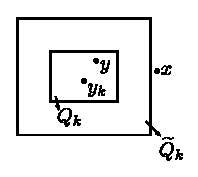
\includegraphics{vol70-figures/fig2.eps}}
\end{figure}

First consider the case $\epsilon =1$. Now $k_1 (z)$ is a
$C^{\infty}$ function which is homogeneous of degree $-n$ for large
$z$. Therefore,  $| grad k_1 (z) | \leq c'' |z| ^{-n-1}$. By the mean
value theorem, 
\begin{align*}
  |k_1  (z-w) - k_1 (z) | & \leq c' |w| \sup_{0< t< 1} |z - tw|^{-n-1}\\
  & \leq c'' |w|| z| ^{-n-1} \text{for} |z| > 2 |w|.
\end{align*}

So
\begin{align*}
  \int\limits_{|z| > 2 |w|} & |(k_1 (z-w) - k_1 (z))| dz\\
  & \leq c''  \int\limits_{|z| > 2 |w|} |w| |z| ^{-n-1} dz\\
  & \leq c''' |w| \int\limits_{2|w|}^{\infty} r^{-2} dr =c.
\end{align*}

Now for general $\epsilon$,
$$
k_{\epsilon} (z) = (1 - \phi (z/\epsilon)) k (z / \epsilon)
\epsilon^{-n}~\text{ by the homogeneity of  }~ k. 
$$

Therefore, if we set $z' = \epsilon^{-1} z$ and $w' =
\epsilon^{-1} w$, we see that 
$$
 \int\limits_{|z| > 2 |w|} |(k _{\epsilon}(z-w) - k
 _{\epsilon}(z))| dz =\int\limits_{|z'| > 2 |w'|} |(k_1 (z' -
 w')-k_1 (z'))| dz' 
 $$
 which is bounded by a constant,  by the result for $\epsilon =1$.
 Hence the \textit{claim} above is proved. 
 
 To\pageoriginale complete the picture,  we should observe that operators of type
 $0$ are not bounded on $L^1$ (and hence,  by duality, not bounded on
 $L^\infty$). Indeed,  if $T$ is an operator of type $0$ with kernel
 $k$, $(Tf)\hat{~} = \hat{k} \hat{f}$.  Since $\hat{f}$ is homogeneous
 of degree $0$, it has a discontinuity at $0$ (unless $k = c
 \delta$). Thus if $f \epsilon L^1, (Tf)\hat{}$ is  not continuous
 at $0$ whenever $\hat{f} (0) \neq 0$ and this implies that $Tf$ is
 not in $L^1$. 
 
 This reflects the fact that if $\int f = \hat{f} (0) \neq 0$, then
 $Tf$ will not be integrable near $\infty$,  because $k$ is itself not
 integrable at $\infty$. However,  there are also problems with the
 local integrability of $Tf$ caused by the singularity of $k$ at the
 origin.  In  fact, let $\phi \epsilon C^\infty_{o}$ be a radial
 function such that $\phi =1$ near 0,  and set $Sf = f * (\phi k)$.
 Then the argument used to prove Theorem \ref{chap5:thm5.16} shows that $S$ is
 bounded on $L^p$ for $1 < p < \infty$.  In this case $(\phi k) \hat{~}
 =  \hat{\phi} * \hat{k}$ is in $C^\infty$,  but still $S$ is not
 bounded on $L^1$. 
 
 This follows from the following general fact.

\setcounter{prop}{19}
 \begin{prop}%pro 5.20
   If $k \epsilon S'$ and the operator $ f \to k * f$ is bounded
   on $L^1$,  then $k$ is necessarily a finite Borel measure.  
 \end{prop}

\begin{proof}
   Choose $\phi \epsilon C_o ^\infty$ with $\int \phi =1$ and put
   $\phi _{\epsilon} (x) = \epsilon^{-n} \phi (x /
   \epsilon)$. Then $|| \phi _{\epsilon}||_1$ is independent of
   $\epsilon$,  so $|| \phi _{\epsilon} * k ||_1 \leq c$.
   Therefore there exists a sequence $\epsilon_{k}$ tending to $0$
   such that $\phi _{\epsilon_k} * k$ converges to a finite Borel
   measure $\mu$ in the weak* topology of measures and hence
   $\phi_{\epsilon_k}* k$ converges to $\mu$ in $S'$ also.  On the
   other hand, since $(\phi _{\epsilon_k})$ is an approximate
   identity, $\phi_{\epsilon_k} * k$ converges to $k$ in $S'$. 
\end{proof}  

Hence\pageoriginale $\mu = k$ and the proposition is proved.

It is easy to see that kernels of type 0 are not measures even when
truncated away from the origin, as their total variation in any
neighbourhood of 0 is infinite. One can also see directly that they
do not define bounded functionals on $C_o$. 

\begin{exercise} 
  Let $k (x) = 1/x$ on $\mathbb{R}$ and let $f$ be a
  continuous compactly supported function such that $f(x) = (\log
  x)^{-1}$ for $0 < x < \dfrac{1}{2}$ and $f(x) =0$ for $x \leq 0$. Show that  
  $$
  \lim_{x \to 0-} (f * PV (k) ) (x) = \infty.
  $$
\end{exercise}

Generalise this to kernels of type $0$ on $\mathbb{R}^n, n > 1$.

This example also shows that operators of type $0$ do not map
continuous functions into continuous functions. However, they do
preserve Lipschitz or H\"{o}lder continuity, as we shall now see. 

\setcounter{defi}{20}
\begin{defi}\label{chap5:def5.21}%def 5.21
  For $0< \alpha < 1$, we define $|f|_\alpha = \sup_{x,y} \dfrac{|f
    (x+y) - f (x)|}{|y|^\alpha}$ 
  $$
  \Lambda_{\alpha} = \{ f: || f ||_{\Lambda_{\alpha}} =^{def} || f ||
  _{\infty} + | f | _{\alpha} < \infty \}. 
  $$
  $\Lambda_{\alpha}$ is called {\em Lipschitz class} of order $\alpha$.
\end{defi}

\setcounter{rem}{21}
\begin{rem}\label{chap5:rem5.22} %rem 5.22
  The definition makes perfectly good sense for $\alpha =1$ (When
  $\alpha > 1$ it is an easy exercise to show that if $|f|_{\alpha}<
  \infty$ then $f$ is constant ). However, we shall not use this
  definition for $ \alpha = 1$, because the theorems we wish to prove
  are false in this case. 
\end{rem}

We are going to prove, essentially, that operators of type $0$ are
boun\-ded on $\Lambda_{\alpha}$. However, if $k$ is a kernel of type
$0$ and $f \epsilon \Lambda_{\alpha}$, the\pageoriginale integral defining $k* f$
will usually diverge $f$ need not decay at $\infty$. Consequently, we
shall work instead with $\Lambda^{\alpha } \cap  L^p (1 < p <
\infty)$, concerning which we have the following useful result. 

\setcounter{prop}{22}
\begin{prop}\label{chap5:prop5.23}%pro 5.23
  If $f \epsilon L^p, 1 \leq p < \infty $ and $|f|_{\alpha}<
    \infty$, then $f \epsilon \Lambda_{\alpha} $ and $|| f ||
    _{\infty} \leq c (|| f || _p + |f|_{\alpha})$. Consequently,  $L^p
    \cap \Lambda_{\alpha}$ is a Banach space with norm $|| f || _p + |f|
    _{\alpha}$. 
\end{prop}

\noindent \textit{Proof.}
  Let
  $$
  A_x = (\frac{|f(x)|}{2 |f|_{\alpha}})^{1/\alpha} \text{ for } x
  \epsilon \mathbb{R}^n. 
  $$
    
  Then $|f (y)| \geq |f (x) |/2$ for all $y$ such that $|x-y| \leq A_x$.  So 
  \begin{align*}
    \int | f (y)|^p dy & \geq  \int\limits_{|x-y|\leq A_x} |f (y) |^p dy
    \geq |f (x) |^p 2^{-p}c' A^n_x\\ 
    & = c'' |f(x)| ^{p+(n / \alpha )} |f| _{\alpha}^{-n/\alpha}
  \end{align*}
  $$
  \displaylines{\text{or}\hfill
  |f (x)|^{1+ (n / \alpha p)} \leq c''' || f ||_p |f|_{\alpha }^{n
    /alpha p}.\hfill\Box} 
  $$

Since this is true for all $x$, setting $\theta = n / p \alpha$ we have 
\begin{align*}
  || f || _{\infty} & \leq c''' || f || _{p}^{1/ (1+\theta )} |f |
  _{\alpha}^{\theta/ (1+\theta )}\\ 
  & \leq c (|| f || _p + |f |_\alpha).
\end{align*}

\setcounter{thm}{23}
\begin{thm} \label{chap5:thm5.24}%the 5.24
  Operators of type $0$ are bounded on $\Lambda_\alpha \cap L^p ( 0
  < \alpha < 1, < 1 < p < \infty)$. 
\end{thm}

\begin{proof}
   Let $T : f \to K *f$ be an operator of type $0$. Since  we know
   that $|| Tf || _p \leq c_p || f || _p$, by
   proposition \ref{chap5:prop5.23}, it
   will suffice to show $|Tf|_{\alpha} \leq c_\alpha |f|_\alpha$\pageoriginale for
   $0< \alpha < 1,  f \epsilon L^p \cap \Lambda_{alpha}$. As in the
   proof of Theorem \ref{chap5:thm5.16}, we may assume that $K = PV (k)$ and
   identify $K$ with $k$. 
\end{proof}

Given $y \epsilon \mathbb{R}^n \backslash \{0\}$ and $f \epsilon L^p
\cap \Lambda_{\alpha}$ define 
\begin{align*}
  g(x) & =  \int\limits_{|z| \leq 3 |y|} k (z) f (x-z) dz\\
  h(x) & = \int\limits_{|z| \leq 3 |y|} k(z) f (x-z) dz
\end{align*}
so that $Tf = g+h$. Since $\mu_k =0$, we have
\begin{align*}
|g(x)| & = | \int\limits_{|z| \leq 3 |y|} k(z) (f (x-z) - f (x) ) dz |\\
& \leq \int\limits_{|z| \leq 3 |y|} c |z|^{-n} |f|_{\alpha} |z|
^{\alpha} dz \leq c_1 |f|_{\alpha} |y|^{\alpha}. 
\end{align*}

Since this is true for all $x$,
$$
|g (x+y)- g(x) | \leq 2 c_1 |f|_{\alpha} |y|^{\alpha}.
$$

Next 
\begin{align*}
  h(x+y) & = \lim\limits_{\eta \to \infty} \int\limits_{3|y| <  |z|<
    \eta} k(z) (f (x+y-z) - f (x)) dz\\ 
  & = \lim\limits_{\eta \to \infty }\int\limits_{3|y| < |z+y|< \eta}
  k(z+y)(f (x-z) -f (x) ) dz. 
\end{align*}

Therefore,
$$
h (x+y) - h (x) = \lim_{\eta \to \infty} \int\limits_{3|y| < |z| <
  \eta} (k(z+y)- k(z)) (f(x-z) -f(x))dz + \epsilon_1 +
\epsilon_2 
$$
where $\epsilon_{1}$ and $\epsilon_2$ are errors coming from
difference between the regions of integration. 

$\epsilon_1$ is the error coming from the difference between the
regions $|z| < \eta $ and $|z+y| < \eta$. 

The\pageoriginale symmetric difference between these two regions is contained in the
annulus $\eta - |y| < |z| < \eta + |y|$. 

\begin{figure}[H]
\centering{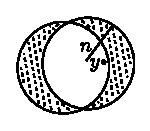
\includegraphics{vol70-figures/fig3.eps}}
\end{figure}

If $z$ is in this region and $\eta \gg |y| $ then $|z| \approx | z +
y| \approx \eta $ so  that 
\begin{multline*}
  |\epsilon_1| \leq c' \int\limits_{\eta -| y | < |z| < \eta + |y|} 2
  \eta ^{-n} || f ||_{\infty} dz \leq c'' \eta ^{-n} || f || _{\infty}
  ((\eta + |y|)^n - (\eta - |y|)^n )\\
  = 0 (\eta^{-1}) \to 0 ~\text{as}~ \eta \to \infty. 
\end{multline*}

The term $\epsilon_2$ comes from the symmetric difference of the
regions $|z| > 3 |y|$ and $| z+y| > 3 |y|$ which is contained in the
annulus $2 |y| < |z| < 4 |y|$. 

In this region $| z + y| \approx |z| \approx |y|$.

Therefore
\begin{align*}
  |\epsilon_2| & \leq c''' \int\limits_{2 |y| < |z| < 4 |y|}
  |y|^{-n+\alpha} |f|_{\alpha} dz =\\ 
  & = c'_2 |f| _\alpha |y| ^{-n+\alpha} ((4| y| )^n - (2 |y|)^n)\\
  & = c_2 |f|_{\alpha} |y| ^{\alpha}.
\end{align*}

Finally coming to the main term, we have 
\begin{align*}
  |k (z + y)- k (z) | & \leq |y| \sup_{0< t< 1} |~\text{grad}~ k (z + ty)|\\
  & \leq |y| \sup_{0< t< 1} |z + ty|^{-n-1}\\
  & \leq c_o |y| |z|^{-n-1} ~\text{for}~ |z| \geq 3 |y|.
\end{align*}

Hence,\pageoriginale since $\alpha < 1$ so that $-n -1 + \alpha < -n$, 
\begin{align*}
  |  \int\limits_{3 |y| < |z| < \eta} & (k (z+y) - k (z) ) (f (x-z) - f(x)) dz | \\
  & \leq c_o \int\limits_{3 |y| < |z| < \eta} |y| |z|^{-n-1}
  |f|_{\alpha} |z|^{\alpha} dz\\ 
  & \leq c_o \int\limits_{3 |y| < |z|} |y| |z|^{-n-1+\alpha} |f| _{\alpha} dz\\
  & \leq c_3 |y| |f|_\alpha |y| ^{\alpha -1} = c_3 |y|^{\alpha} |f|_{\alpha}.
\end{align*}

Therefore,
$$
\frac{|Tf (x+y) - Tf (x)|}{|y|^{\alpha}} \leq c |f|_{\alpha} \text{and
  consequently } |Tf | _{\alpha} \leq c |f|_{\alpha}. 
$$

For kernels of positive type, we have the following result.

\setcounter{thm}{24}
\begin{thm}\label{chap5:thm5.25}%the 5.25
  Suppose $ 0 < \lambda < n,  1 < p < n/\lambda < q < Q$ where $Q
    = \infty $ if $ \lambda \leq 1,  Q = n/ (\lambda-1)$, if $\lambda
    < 1$.  Let $ 1/r = (1/p) - (\lambda /n)$ and $\alpha = \lambda -
    (n/q)$.(Thus $r < \infty$ and  $ 0 < \alpha < 1$). Thus operators
    of type $\lambda$ are bounded from $L^p \cap L^q$ into $L^r \cap
    \Lambda_{\alpha}$. 
\end{thm}

\begin{proof}
  Let $Tf = k * f$ be an operator of type $\lambda$. By Corollary
  \ref{chap5:coro5.15}, $T$ is bounded from $L^p $ to $L^r$, so by
  proposition \ref{chap5:prop5.23}, 
  it is enough to show that $|Tf|_{\alpha} \leq c || f || _q$. 
  \begin{align*}
    \text{We have } (Tf) (x) & = \int f (x-z) k (z) dz\\
    (Tf) (x+y) & = \int f (x + y -z) k (z) dz\\
    & = \int f (x-z) k (z+y) dz,
  \end{align*}
  so that
  \begin{align*}
    (Tf) (x+y) - Tf (x) & = \int f (x-z) (k (z+y) - k (z)) dz\\
    & = \int\limits_{|z| \leq 2 |y|} f (x-z) (k (z + y)- k (z)) dz\\
    & \quad +\int\limits_{|z| > 2 |y|} f (x-z) (k (z+y) - k (z)) dz. 
  \end{align*}\pageoriginale
\end{proof}

If $q'$ is the conjugate exponent of $q$,
\begin{align*}
  |\int\limits_{|z| \leq 2 |y|} & f (x-z)(k (z+y) - k (z) ) dz|\\
  & \leq || f || _q \left\{ \left(~ \int\limits_{|w| \leq 3 |y|} | k(w)^{q'} dw
  \right)^{1/q'} +  \left(~\int\limits_{|z| \leq 2 |y|} | k (z)^{q'}
  dz\right)^{1/q'} \right\} \\ 
  & \leq 2 || f || _q \left(~\int\limits_{|z| \leq 3 |y|} | k (z)
  |^{q'} dz \right)^{1/q'} \\
  & \leq c_1 || f ||_q \left(~ \int\limits_{|z| \leq 3 |y|} |z|^{ (\lambda -
    n)q'} dz\right) ^{1/q'}\\ 
  &\leq c'_1 || f ||_q |y|^{-n + \lambda + (n/q')} = c'_1 || f || _q |y|^\alpha,
\end{align*}
by the definition of $\alpha$

For the second integral, we estimate $k(z+y) - k(z)$ by the mean value theorem:
\begin{align*}
  |k (z+y) - k (z)| & \leq |y| \sup_{0< t<1} | \text{grad} k (z+ty)|\\
  & \leq c |y||z| ^{\lambda - n -1} \text{for } |z| \geq 2 |y|.
\end{align*}

Thus
\begin{align*}
|\int\limits_{|z| > 2 |y|} & f (x-z) (k(z+y)- k(z)) dz|\\
  & \leq c || f || _q \left\{ ~\int\limits_{|z| > 2 |y|}\left(|y| |z|
  ^{\lambda-n-1}\right)^{q'}dz \right\}^{1/q'}\\ 
  & \leq c'_2 || f || _q |y| |y|^{\lambda - n-1+ (n/q')} ~\text{since}~
  (\lambda -n-1)q' < - n\\ 
  & = c'_2 || f || _q |y|^{\alpha}.
\end{align*}

Hence\pageoriginale 
$$
\frac{|Tf (x+y) - Tf (x)|}{|y|^{\alpha}} \leq c || f || _q ~\text{which
  gives}~ | Tf |_{\alpha} \leq c || f || _q. 
$$

\setcounter{rem}{25}
\begin{rem}\label{chap5:rem5.26}%rem 5.26
  As in the preceding theorem, the reason for taking the domain of $T$
  to be $L^p \cap L^q$ instead of just $L^q$ is that the integral
  defining $Tf$ will usually diverge when $f$ is merely in $L^q$. 
\end{rem} 


Nonetheless, the point of these theorems is that operators of type 0
are in essence, bounded from $L^q$ to $\Lambda_{\alpha}$ (for
appropriate $q$ and $\alpha$). To make this precise without losing
simplicity, one can observe that operators of type $ 0$ map
$\Lambda_{\alpha} \cap E'$ into $\Lambda_{\alpha}$ while operators of
type  $\lambda > 0$ map $L^q \cap E'$ into $\Lambda_{\alpha}$. 

We now introduce spaces of functions whose derivatives upto a certain
order are in $L^p$ or $\Lambda_{\alpha}$. 

\setcounter{defi}{26}
\begin{defi}\label{chap5:def5.27}%def 5.27
  Suppose $1 \leq p \leq \infty$ and $k$ is a positive integer.  We define
  $$
  L^p_k = \{ f : D^{\beta} f \epsilon L^p \text{for} 0 \leq |\beta| \leq k\}.
  $$
\end{defi}

We equip $L^p_k$ with the norm $|| f || _{k,p}= \sum\limits_{|\beta|
  \leq k} || D^{\beta}f ||_p$. (Thus $L^2_k = H_k$ in the notation of
Chapter \ref{chap3}). 


\begin{defi}\label{chap5:def5.28}%def 5.28
  Suppose $k$ is a positive integer and $k < \alpha < k + 1$. We define
  $$
  \Lambda_{\alpha} = \{ f : D ^{\beta} f \epsilon \Lambda_{\alpha -
    k} \text{for} 0 \leq |\beta| \leq k\}. 
  $$
\end{defi}

We equip $\Lambda_{\alpha}$ with the norm $|| f || _{\Lambda_{\alpha}}
= \sum_{|\beta| \leq k} || D^{\beta} f ||_{\Lambda_{\alpha - k}}$. 

\setcounter{remarks}{28}
\begin{remarks}\label{chap5:rem5.29}%rem 5.29
~

  \noindent (i)~ $f \epsilon \Lambda_{\alpha}$\pageoriginale if and only if
    $D^{\beta} f$ is 
    bounded and continuous for $ 0 \leq |\beta| \leq k$ and $D^{\beta }
    f \epsilon \Lambda_{\alpha -k}$ for $|\beta| =k$. Indeed, if
    $|\beta| < k$, for $|y | \leq 1$, 
    $$
    \frac{|D^{\beta} f (x+y) - D^{\beta} f (x)|}{ |y|^{\alpha -k}} \leq
    \frac{|D^{\beta} f (x+y) - D^{\beta} f (x)|}{|y|} \leq c\sum_{|v| =
      |\beta| +1} || D^v f ||_{\infty} 
    $$
    (by the mean value theorem) and for 
    $$
    |y| > 1, \dfrac{|D^{\beta} f
      (x+y) - D^{\beta} f (x)|}{ |y|^{\alpha -k}} \leq 2 || D^{\beta } f
    ||_{\infty}.
    $$ 
  
    This shows that $D^\beta f \epsilon \Lambda_{\alpha -k} $ for
    $0\leq |\beta| \leq k $ i.e., $f \epsilon \Lambda_{\alpha}$. 
    
    \noindent (ii)~ If $k < \alpha < k+1$ then $L^p_k \cap \Lambda_{\alpha}$ is a
    Banach space with the norm 
    $$
    \sum_{|\beta| \leq k} (|| D^{\beta} f ||_p + | D^\beta f |_{\alpha -k}).
    $$
    This follows from the corresponding fact that $L^p \cap
    \Lambda_{\alpha}$ is a Banach space (Proposition \ref{chap5:prop5.23}).  
\end{remarks}

\setcounter{thm}{29}
\begin{thm}\label{chap5:thm5.30} %the 5.30
  Suppose $0 \leq \lambda < n,  1 < p < n/\lambda,  1/r = (1/p) -
  (\lambda /n)$ and $k = 0,1,2,\ldots$. Then we have:  
  \begin{enumerate}[a)]
  \item Operators of type $\lambda$ are bounded from $L_k^p$ into $L^r_k$.
  \item If $\lambda$ is an integer,  $\lambda = 0,1,2,\ldots$ and $k
    < \alpha < k+1$, then operators of type $\lambda$ are bounded from
    $L^p_k \cap \Lambda_{\alpha} $ to $L^r_{k+\lambda} \cap
    \Lambda_{\alpha + \lambda}$.
  \end{enumerate}
\end{thm}

\begin{proof}
  a) This is an easy consequence of Corollary \ref{chap5:coro5.15} and Theorem
  \ref{chap5:thm5.16}, since convolution commutes with
  differentiation. In the  same
  way $(b)$ follows Theorem \ref{chap5:thm5.24} when $\lambda =0$. 
\end{proof}

We now proceed by induction on $\lambda$. Therefore, assume that
$\lambda \geq 1$. Suppose $ f \epsilon L^p_k \cap
\Lambda_{\alpha}$. Then $\partial_j (f * k) = f * \partial _j k$ and
$\partial _j k$ 
is\pageoriginale a kernel of type $\lambda -1$. So, if  $1/s = (1/p)-(\lambda
-1)/n$, by our induction hypothesis $\partial_j(f * k)  \epsilon
L^s_{k+\lambda -1} \cap  \Lambda_{\alpha +\lambda -1}$.  Since $ s < r
< \infty,  L^s \cap L^\infty \subset L^r$,  so  $\partial_j ( f * k)
\epsilon L^r_{k+\lambda -1} \cap   \Lambda _{\alpha + \lambda
  -1}$. Also $f * k \epsilon L^r \cap C^1$, hence in $ \Lambda
_{\alpha + \lambda}$ provided it is bounded. But $\partial_j(f * k)\in
\Lambda_{\alpha+\lambda-1}$ implies that $\partial_j( f * k)$ is
bounded. By the mean value theorem, we then have 
$$
\frac{ | (f * k) (x+y)-(f * k)(x) | }{ | y  |} \le c.
$$ 

This together with $f * k \epsilon L^r$ implies that $f$ is bounded
(by 
%%%% mistake proposition 5.21
definition \ref{chap5:def5.21}). Hence $ f * k \epsilon L^{r}_{k+\lambda
}\cap  \Lambda_{\alpha + \lambda}$. 

The above theorem can be generalised.  For example, if $0 \le \lambda
< n$ one can show that operators of type $\lambda $ map $ \Lambda
_{\alpha}\cap E'$ in to $ \Lambda_{\alpha +\lambda}$. 

Also generalisations of the $L^p$ Sobolev spaces $L^{p}_{k}$ can be
given for non-integral values of $k$. In fact, a theorem due to
CALDERON says that for $1 < p < \infty, f \epsilon L^p_k$ if and
only if $ \Lambda ^k f \epsilon L^p$. (Here $ \Lambda = (1 -\Delta)
^{1/2}$). 

Therefore, we can define $L^p_s$ for any real $s$ by

$ L^p_s = \{f:  \Lambda ^s f \epsilon L^p\}$ with the norm $ ||  f
||_{s,p}=  ||  \Lambda^s f  ||  _p$. 

Then part (b) of the above theorem is still true for $0 \le \lambda
< n, \lambda$ not necessarily an integer in this case. 

Refer to E.M. Stein \cite{2}.

We will now prove the \textit{ Sobolev imbedding theorem for} $L^p$
\textit{ Sobolev spaces} $L^p_k$ \textit{ with positive integral }
$k$. This theorem can also be generalised\pageoriginale to $L^{p}_{s}$ for $s$ in
$\mathbb{R}$.  

\setcounter{thm}{30}
\begin{thm}[SOBOLEV IMBEDDING THEOREM]\label{chap5:thm5.31} %def 5.31
  Suppose $1 < p < \infty$  and  $k$
  a positive integer.  If  $ k < n/p$,  then  $L^p_k\subset L^r$  for
  $1/r = (1/p) - (k/n)$  (Hence also $L^p_{k+j} \subset L^r_j$  for any
  $j$).  If  $ k > n/p$,  and  $\alpha = k- n/p$  is not integer, then
  $ L^p_k \subset  \Lambda _\alpha$.   
\end{thm}

\begin{proof}
  Let $N$ be the fundamental solution of $\Delta$ given by
  $$
  N(x=)
  \begin{cases}
    (2-n)^{-1} \omega ^{-1}_{n}  | x  | ^{2-n} \text{ for } n \neq 2\\
    (2\pi )^{-1} \log  | x  | \text{ for } n=2.
  \end{cases}
  $$
  Then $K_j(x)=\partial_j N(x)= \omega _n x_j  | x  | ^{-n}$ ( true for
  all $n$) is a kernel of type 1. 
\end{proof}

Now, if $f \in L^p_k \cap E'$

$f= f * \delta = f * \Delta N = f * \sum\limits^{n}_{j=1} \partial _j
k_j = \sum\limits ^{n}_{j=1} (\partial _j f * k_j)$. 

Suppose $k=1$. If $1 < n/p$, $ \partial_j f \epsilon L^p \Rightarrow
 \partial_j f * k_j \epsilon L^r$ where $1/r = (1/p)- (1/n)$, by
 Theorem \ref{chap5:thm5.25} and hence $ f \epsilon L^r$.   If  $1 > n/p,
 \partial _j f * k_j \epsilon  \Lambda _{1-(n/p)}$ by Theorem
 \ref{chap5:thm5.25} which implies that $ f \epsilon  \Lambda _{1(n/p)}$. 
Thus the theorem is true for $k = 1$.

For $k > 1 $, we proceed by induction. Now

$f \epsilon L^p_k \cap E'\Rightarrow f$  and  $ \partial_j f$  are
in $ L^p_{k-1} \cap E'$. 

Therefore, if $ p < n / (k-1)$  and  $1/q = (1/p) - (k-1) / n $, we
have $f$, $\partial_j f \epsilon L^q$, i.e., $f \in L^q _1$,  while
if  $p > n / (k-1)$, we have $f$, $ \partial_j f \epsilon  \Lambda
_{k-1-(n/p)}$, i.e., $f \epsilon  \Lambda_{k-(n/p)}$. In the second
case, we are done, and in the first case, we apply the result for
$k=1$ to see that $f$ is\pageoriginale in the required space. Finally, it is easy to
check that if we keep track of the norm inequalities that are implicit
in the above arguments, we obtain 
$$
 ||  f  ||_r \le c  ||  f  ||_{k,p} ~\text{ or }~  ||  f   ||_{
   \Lambda_\alpha} \le c  ||  f  ||_{k,p}, 
$$ 
as appropriate, for $ f \epsilon L^p_k \cap E'$.  Since $L^p _k \cap
E'$ is clearly dense in $L^p_k$, the desired result follows
immediately. 

We can summarise these theorems in an elegant way using the following
picture. 

For $ - n < \alpha < 0$ we define $x_\alpha = L^{n/ | \alpha |}$ and
when $\alpha > 0$, $\alpha$ not an integer, we define $x_\alpha =
\Lambda_\alpha$.  

\begin{figure}[H]
\centering{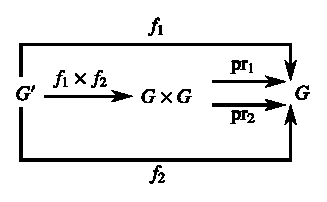
\includegraphics{vol70-figures/fig4.eps}}
\end{figure}
(The small circle represent missing spaces)

In this terminology, we have

\setcounter{thm}{31}
\begin{thm}\label{chap5:thm5.32}%the 5.32
  Operators of type $\lambda$  map  $ x_\alpha \cap E'$  into  $
  x_{\alpha+\lambda} o \le \lambda < n$. 
\end{thm}

\begin{thm}[SOBOLEV IMBEDDING THEOREM] \label{chap5:thm5.33}% the 5.33
  If $D^\beta f \epsilon x_\alpha $
  for  $ 0 \le  | \beta  | \le k$,  then  $f \in x_{\alpha + k}$. 
\end{thm}

We now indicate how to fill the gaps in this picture at $\alpha = 0, 1
, 2, \ldots$ 

For $\alpha = 1$, we define 

$ \Lambda_1 = \{f:f$ is continuous, bounded and 
$$
\sup_{x,y} \frac{ | f(x+y) + f(x-y) - 2f(x) | }{  | y  | } < \infty \}.
$$

For\pageoriginale $k= 2,3,4, \ldots$ we define $ \Lambda _k = \{f : D^\beta f
\epsilon \Lambda_1$ for  $| \beta | \le k-1\}$. The sudden jump
from first differences in the definition of $ \Lambda_\alpha$ for
$\alpha < 1 $ to the second differences at      $\alpha =1$ is less
mysterious than it seems at first, because it can be shown that if $ 0
< \alpha < 2$ then $ f \epsilon \Lambda_\alpha$ if and only if $f$
is bounded, continuous and satisfies  
$$
\sup_{x,y} \frac{ | f(x+y) + f(x-y) - 2f(x) |}{ | y |^\alpha} < \infty.
$$  

To fill the gap at $\alpha =0 $ we use the space BMO (`` bounded mean
oscillation'') first introduced by F. JOHN and L. NIRENBERG in
1961, which is defined as follows. 

For $f \epsilon L^1_{\loc} (\mathbb{R}^n)$, we denote by $m_Ef$ mean
value of $f$ over a measurable set $E\subset \mathbb{R}^n$, that is, 
$$
m_Ef = \frac{1}{ | E  |} \int\limits_E f.
$$

Let $\mathcal{Q}$ denote the collection of all cubes in $\mathbb{R}^n$ with sides
parallel to the axes. 

\setcounter{defi}{33}
\begin{defi}\label{chap5:def5.34}%def 5.34
  $BMO = \{f \epsilon L^1_{\loc} (\mathbb{R}^n) : \sup\limits_{Q
    \epsilon \mathscr{Q} } m_Q ( | f - m_Q f  | )< \infty \}$.  
  
  Clearly $L^{\infty} \subset BMO$,  for, $f \epsilon L^\infty
  \Rightarrow  | m_Q f  | \le  ||  f  ||_\infty$ for every $Q
  \epsilon \mathscr{Q}$ and consequently 
  $$
  m_Q ( | f - m_Q f  | ) \le  2 ||  f  ||_\infty.
  $$
\end{defi}

It can be shown that $BMO \subset L^q_{\loc}$ for every $q < \infty$.

If we define $x_\alpha =  \Lambda_\alpha$ for $ \alpha = 1,2,  \ldots$
and $X_0 = BMO$ then Theorem \ref{chap5:thm5.32} remains valid for all
$\alpha_{\epsilon} (-n, \infty)$, except that the Sobolev
imbedding theorem for $\alpha = 0$ must be slightly modified as
follows:  

If\pageoriginale $D^\beta f$ is in the closure of BMO $\cap E'$ in BMO for $ |
\beta | \le k$ then $ f \epsilon \Lambda_k$. 

\begin{warning}
  BMO  is not an interpolation space between $L^p$ and $ \Lambda
  _\alpha$ i.e., it is not true that if $T$ is a linear operator which
  is bounded on $L^p$ for some $p < \infty$ and on $ \Lambda_\alpha $
  some $\alpha > 0$, then $T$ is bounded on BMO. 
\end{warning}

For proofs of the foregoing assertions, see E.M. Stein [$2$] and also
the following papers : 
\begin{enumerate}[(i)]
\item E.M Stein and A. Zygmund: Boundedness of translation invariant
  operators on Holder spaces and $L^p$ spaces, Ann. Math 85
  (11967)337-349,  and  
\item  C. Fefferman and E.M. Stein : $H^p$ spaces of several variables
  Acta Math. 129,  (1972), 137-193. 
\end{enumerate}

As we indicated at the beginning of this chapter, the arguments we
have developed can be extended in a fairly straightforward way to give
estimates for $\psi DO$ with variable coefficients. We conclude by
summarising the result in  

\setcounter{thm}{34}
\begin{thm}\label{chap5:thm5.35}%5.35
  [Let] $P=p(x,D)$ ba a properly supported  $\psi DO$ of
    order  $-\lambda $  on  $\Omega $, where  $\lambda
  \ge 0$  and  $p \sim \sum\limits^{\infty}_{j=0} p_j$ 
    with  $p_j(x, \xi)$ homogeneous of degree  $\lambda - j$ 
       for large  $ | \xi  | $.  Then  $P$ maps $L^p_k
      (\Omega, \loc)$ into $L^p_{k+\lambda}(\Omega,  \loc)$ 
      for  $1 < p < \infty$,  and in the terminology of Theorem
        \ref{chap5:thm5.32}  $P$  maps $x_\alpha (\Omega,  \loc)$  into
       $x_{\alpha + \lambda}(\Omega, \loc)$ for $- n < \alpha
      < \infty $. 
 \end{thm}
 
\begin{thebibliography}{99}
\bibitem {1} { G. B. FOLLAND}:\pageoriginale Introduction to partial differential
  equations Princeton University press, Princeton, N. J., 1975. 
\bibitem {2} {E.M. STEIN }: Singular integrals and differentiability
  properties of functions, Priceton University press, Princeton, N.J.,
  1970. 
\bibitem {3} {M. TAYLOR}: (i) Pseudo differential operators,

Lecture Notes in Math \# 416, Springer-Verlag, New York, 1974.
(ii) Pseudo differential operators,
Princeton University press, Princeton, N,J., 1981

\bibitem {4} {F. TREVES}: Basic linear partial differential equations,
  Academic press, New York, 1975. 
\bibitem {5} {A. ZYGMUND} : Trigonometric series, Cambridge University
  press Cambridge, U.K. 1959. 
\bibitem {6} { L. HORMANDER }: Linear partial differential operators,
  Springer-Verlag, New York, 1963. 
\bibitem {7} { W. RUDIN }: Functional Analysis, McGraw-Hill, New York,
  1973. 
\bibitem {8} { F. TREVES }: Topological Vectors spaces, Distributions
  and Kernels, Academic press, New York, 1967. 
\end{thebibliography} 
